\chapter{The lanalytics package}

The \textit{lanalytics package}\footnote{The package is open source and it is hosted on Github. \url{https://github.com/savrgg/lanalytics}} is an R package designed to analyse the answers to online quizzes. The objective of this package is to accomplish one of the main objectives of this text, that was the management and constant analysis of student answers and test times. The package is able to perform different analysis according to the desired grouping level: per quiz, per group and per person. To accomplish this, the data can be plotted in seven different ways, varying on the distinct aggregation levels and the different objectives of the analysis. At the group level, the package contains the \textit{guessing} and the \textit{Time-easiness} plots; at the quiz level, it contains two descriptive statistical graphs, a \textit{boxplot} and a \textit{histogram} of the obtained scores of the online quizzes takers and the \textit{Easiness-Time} and the \textit{Easiness-Time-Level} plots. Finally, at the individual level, the user can plot the grade history of a student. The explanations and objectives of each one of these will be explained throughout this chapter. For all the plots in this chapter, a synthetic dataset was used for illustration purposes; these plots were not generated with any real quiz dataset.

\section{Design of the package}

\subsection{Initial investigation}

Previous work on open source software for analysing quizzes has been done. One of the most popular software is Moodle (Modular Object Oriented Dynamic Learning Environment) that is learning management system \cite{zeileis2012flexible} \cite{moodle}. Which allows creating customisable webpages for the courses. With this tool, the instructors can generate and calculate the grades for their students. Also, it allows the tracking progress of the students. 

Some other user interfaces have been proposed to analyse the data from the students, as student engagement, attendance, and interactions with other students. For example, the Desire2Learn software has tools to achieve a personalised learning and also add-ons that allow analysing the engagement and the performance of the students \cite{desire}. Other software like learning catalytics was designed to increase student engagement  \cite{learningcatalytics}. But, as opposed to Moodle, these two solutions are not freely available.

In the CRAN (Comprehensive R Archive Network) there are some packages that allow the creation and evaluation of exams. One of these tools is the exams2nops function from the \textit{exams} package \cite{zeileis2012flexible}, but according to with the realized research no package was found to manage and analyze quizzes and items of the quizzes in distinct levels that was coded in R. For this reason, the lanalytics package was proposed as a useful tool to produce the required analysis for the instructors.

\subsection{Cognitive levels}

It is important to define the cognitive levels that are used in this package. These levels are based on the levels of the Bloom's taxonomy (remember, understand, apply, analyse, evaluate, create) \cite{Bloom1956}. The first level that we defined for this analysis include the easiest questions, those that only implies a \textit{factual knowledge}. These are questions that only require memorising and repeat the definition of a concept. The second level is the \textit{understanding of the concept}, where the student should not only know the definition but also to be able to discuss it and explain it. In the last level, \textit{application of concept}, the student should know how to execute and operate the concept in real problems or situations \cite{Stefan2015b}.

\subsection{Quiz and course objects}

To allow the instructors to manage the quizzes and course data, the lanalytics package created two exportable objects, the quiz object, and the course object. The basic structure of the lanalytics package is the quiz object which is implemented with a \textit{tibble} \cite{wickham2016r} \footnote{A tibble is data structure build on top of the data.frame class and give it more functionalities.}. This object contains a tibble in long format with one entry per student-question. For each row, another two variables are required: the score (a binary variable indicating if the answer was correct) and the date-time when the question was answered (in \textit{POSIXct} format). All this information should be provided in a \textit{*.csv} file. 

To allow more interesting analysis, the quiz object can be augmented with other two columns computed by R. The first is the spent time per question and the second is the answering order (a number is assigned to each row according to the order in which it was answered). An example of the quiz object is in the [\cref{img:quiz_object}]. 

\begin{figure}[ht!]
  \centering
  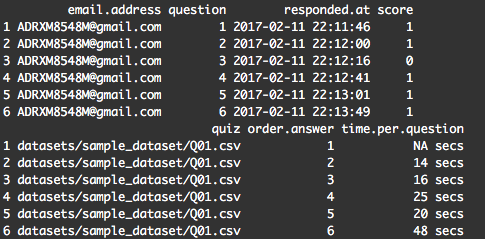
\includegraphics[width=.75\linewidth]{img/quiz_object.png}
  \caption{Quiz object. It has an specified format and columns.}
  \label{img:quiz_object}
\end{figure}

Finally, all the quizzes can be grouped in a course object, which joins them in the same tibble. This is very useful if the instructors want to save the all the records of their course in just one file.

\section{Group level analysis}
The group level analysis can potentially help the instructors to monitor the performance of all the group through all the course. Different interesting aspects of the group are analysed in this section. First, a guessing plot that helps to detect which potentially students that are answering randomly or with some exterior help is presented. After this, an Easiness-Time plot per time-terciles is made, in which the main objective is to understand in general how the group is answering the quiz regarding time. Also, the relation between this invested time and the obtained score in the items is presented. This tab was created to help the instructors to understand all the group behaviour in the quiz (for the guessing plot they can quickly observe the all the anomalous behaviours in the group and for the easiness time per quiz they can observe how the students are answering the questions according to the time).

\subsection{Guessing plot}

The idea of the \textit{guessing plot} \cite{Stefan2015b} [\cref{img:group_guess}] is to detect if a student is answering the questions in a very fast pace. Some students can answer the quizzes fast, but even the fastest of them answer the questions above some time threshold. This threshold is relative to the item difficulty and the student's ability, so one way to find a lower bound is to insert a question that every student can answer almost immediately in some section of the quiz and record the time that each student spends on it (For example, an easy a fast question can be: "did you attend this week's lecture?"). If some other question is answered below this time threshold, then it should be analysed. As the fast question answering does not give more information about the student behaviour (the student could be answering randomly or could know the answer from another student), the obtained score should be analysed. In the guessing plot if someone spends less time than the threshold, then a point will appear. If the answer was correct, then the colour of the point will be red. Otherwise, it will be blue.

\begin{figure}[ht!]
  \centering
  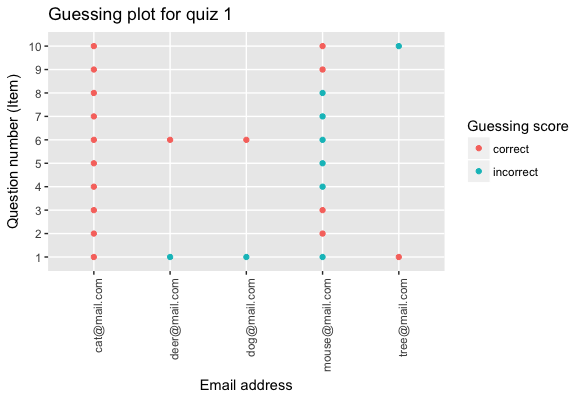
\includegraphics[width=.9\linewidth]{img/group_guess.png}
  \caption{Guessing plot. A point indicates that the user answers the item faster than some threshold. If it is red, the answer is correct, otherwise is incorrect.}
  \label{img:group_guess}
\end{figure}

The intuition of this plot is that, if the student gets many red points in the same quiz, it is possible that the answers to the items were known previous to the quiz. If the student gets many red and blue points, it is possible that the quiz was answered just randomly. The ideal situation is that no or just a few points appear per student in the graph. For example, in the \cref{img:group_guess} we have 5 users. The users \textit{cat@mail.com} and the user \textit{mouse@mail.com} answered fast all the questions, but the difference is that the user \textit{cat@mail.com} got every question correct while the other user does not. Because of the defined threshold, it is possible that the first student previously knew the answers, while the second one just answers randomly.


\subsection{Easiness time per quiz and tercils}

In the Easiness-Time plot \cref{img:group_order} the students are grouped by tertiles according to the time that they spent in the question. This way, the first tercile contains the fastest students and the third tercile the slowest. The intuition behind this plot is that, if both the fast and slow answering students score correctly in some question, then it is an easy one. On the other hand, if there is a score gap between the fast and slow students, then it may be interpreted differently. If the fast-answering students get a better result, then it may be interpreted as they know the solution, so they answer it faster. On the other hand, if the slow-answering students have a better result, this item might be a little bit confusing, so the students spend more time trying to figure out the solution.

\begin{figure}[ht!]
  \centering
  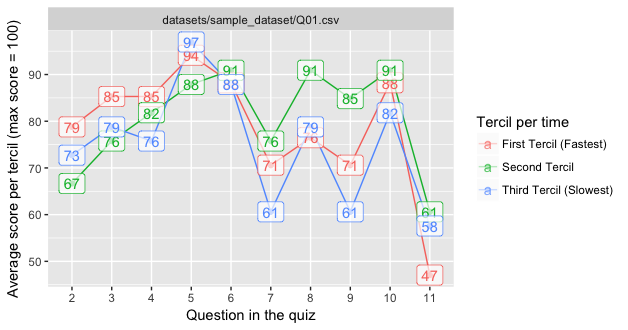
\includegraphics[width=\linewidth]{img/group_order.png}
  \caption{Easiness-Time per group and tercil. In the x-axis is the question of the quiz and in the y-axis the average score per time-tercil.}
  \label{img:group_order}
\end{figure}

In the \cref{img:group_order} we can see these patterns. For example, in the questions 5 and 6, all the students got an average of 90. Conversely, in the questions 2,3,4, the faster students got better results than, the slower ones.

\section{Quiz level analysis}

The quiz level analysis can potentially help the instructors to monitor the performance and analyse the data quickly from the perspective of the quiz and items. Different aspects that can be evaluated from this are the easiness of the items and the median spent time in each one of them \footnote{It has calculated the median so that the analysis is not affected by outliers}. First, to give a general idea of the performance of the students in the selected quiz, a histogram and a boxplot of the scores are displayed. This can help to analyse the outliers and the dispersion of the data. After these, two plots analyse the items from a perspective of easiness and time. Conversely to the Easiness-Time plot of the group level, here we are interested in the general performance of the quiz. We would like to observe that difficult items take more time than easy ones, so there is a negative relation between easiness and time. This point can be addressed with the ET-plot \cite{Stefan2015b}. Additionally, we would like to see if this easiness is related with the cognitive level, as intuitively, a higher cognitive level requires more time (For example, to apply a concept, first the student should understand it and remember it).

\subsection{Histogram of quizzes}

To identify the dispersion and skewness of the data we can analyse the histograms per quiz. With these is easy to detect if there are subpopulations in the data (for example if the distribution is similar to a bimodal normal distribution). In the [\cref{img:quiz_hist}] the quiz 01 looks normally distributed, and the quiz 02 looks like a bimodal distribution.

\begin{figure}[ht!]
  \centering
  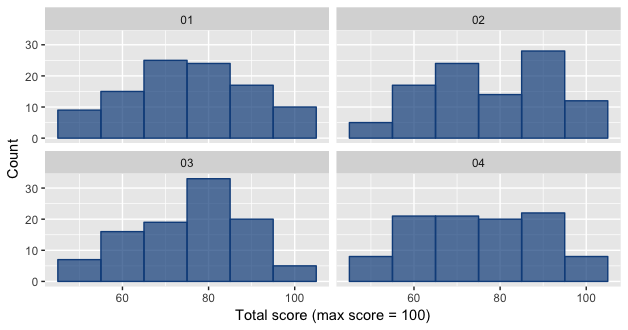
\includegraphics[width=.85\linewidth]{img/quiz_hist.png}
  \caption{Quiz scores histogram. In this plot four quizzes are displayed.}
  \label{img:quiz_hist}
\end{figure}

\subsection{Boxplot of quizzes}

Another way to verify the distribution and the skewness of the data is to analyse the boxplots of the scores. A useful aspect of these plots is that they allow us to detect outliers. This is important because the instructor can detect how many students are performing badly or well (depending on what kind of outlier is presented). After that, the instructor can only spend time analysing these points individually and see what topics are confusing for them.

The implemented boxplot in the ggplot2 package \cite{ggplot2} is the Tukey boxplots \footnote{Basically the other types of boxplots differ in the way that the whiskers are constructed.}, which use the first and third quartile as the hinges and limit the length of the whiskers to 1.5 of the interquartile IQR length. If a point in the data is outside these ranges, then it is classified as an outlier. For the upper whisker, if the value is greater than the maximum value of the data, then the whisker is reduced to this value (An equivalent rule apply for the lower whisker). 

\begin{figure}[ht!]
  \centering
  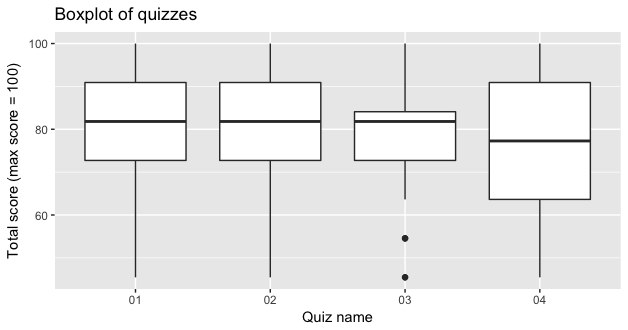
\includegraphics[width=\linewidth]{img/quiz_boxplot.png}
  \caption{Quiz scores boxplot (Also called box and whiskers diagram). This plot display five different summary statistics: median, two whiskers and two hinges. In addition the plot display the outlier points.}
  \label{img:quiz_boxplot}
\end{figure}

For example, in the boxplot of the \cref{img:quiz_boxplot} we can see that the lower whisker of the quiz 03 is much smaller than the other quizzes and, as seen in the histogram of the quiz 03, we can identify that this distribution has a much bigger mode than the other 3. As a consequence, the 50\% of the data is in contained in a smaller interval, which is reflected in its boxplot.

\subsection{Easiness-Time plot}

The objective of the Easiness-Time plot (ET plot) is to analyse the relationship between the required time for each item versus the average score obtained in the corresponding item. In the quiz design, it is important to consider the required time that each student should spend on each item, this way the instructor can design quizzes according to some pre-established time and discrimination criteria. With this plot, the instructor can analyse both points. Also, a tendency line is displayed in the plot.\footnote{To avoid overlay in the labels of the points; the ggrepel package was used.}.

\begin{figure}[ht!]
  \centering
  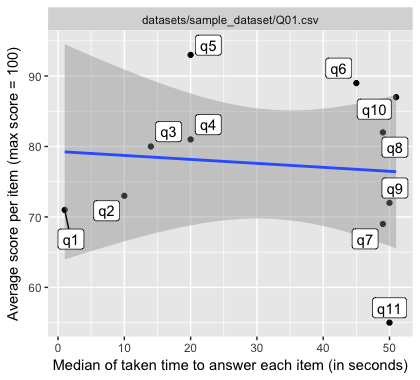
\includegraphics[width=.75\linewidth]{img/quiz_et.png}
  \caption{Easines-Time plot}
  \label{img:quiz_et}
\end{figure}

For example, in the \cref{img:quiz_et} we can see that question 5 is taking 20 seconds to answer (an intermediate time in this example), but the students achieve a high average score. On the other hand, the question 11 is taking too long for the students, and many of them get it wrong. Then, the instructor can examine why the students are getting wrong the question (because it seems that it is not a matter of time).

\subsection{Easiness-Time-Level plot}

The ETL plot \cite{Stefan2015b} adds the extra layer of the cognitive level to the ET plot. As stated at the beginning of the section, in this package we consider three different cognitive levels. The hypothesis is that difficult questions (in the sense of cognitive level) should take more time to answer than the easy ones. If we colour the points by the cognitive level, we might see that the high cognitive levels take in average more time to answer them (because we need to know the concept, then apply it). Moreover, in questions that require a high cognitive level, the students may get a lower score. The reasoning behind this idea is that, if the students don't know the factual knowledge (Low cognitive level), they will not know the application of this concept (High cognitive level), so the score is lower. 

The importance of this plot is to detect the questions where time and difficulty do not align with instructor-rated pre-established cognitive level. For example, if a low cognitive level question is taking too long to be answered, it could mean that this question is being difficult to understand or that the topic, in general, is difficult for the students (For example, in \cref{img:quiz_etl}, the question 6 and 10). Another example is the behaviour represented in question 1. This is a high cognitive question but the student answer it fast, so almost 30\% get it wrong. This can imply that the students have a misconception for the topic related to this question (the students think they know the answer, but they get it wrong). 

\begin{figure}[ht!]
  \centering
  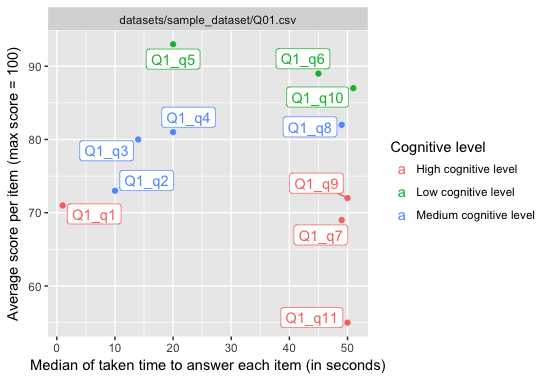
\includegraphics[width=.8\linewidth]{img/quiz_etl.png}
  \caption{Easiness-Time-Level plot.}
  \label{img:quiz_etl}
\end{figure}

\section{Individual plot}

Although the main objective of this package was to provide a way quickly analyse the data for all the group and quizzes, the instructors may be interested in visualising one particular student or group of students. In special if these students were outliers in the group and quiz analysis. This way, they can look for a specific way to support these students. To explore and understand the history of these particular students, an individual history plot is implemented. For this plot, the instructor needs to filter the required students from a list and then observe its history and scores in different quizzes. 

\begin{figure}[ht!]
  \centering
  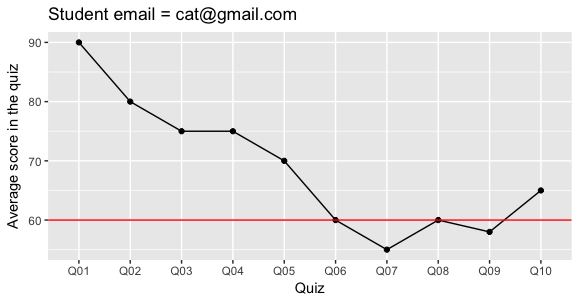
\includegraphics[width=\linewidth]{img/ind_student.png}
  \caption{Individual performance}
  \label{img:ind_student}
\end{figure}

Besides, when the course finishes, the instructor can upload a file with the final grade of the students and observe distinct patterns that can lead to failure of the test. An example of this graph is in the \cref{img:ind_student}. We can see that this student is getting worse in his evaluations, so an opportune instructor intervention in an early stage of the course could improve the student's performance on the final exam.

\section{Documentation}
Finally, the documentation is important for the package. For this reason, two different ways to make the documentation were compared. The first way, the codes were commented manually and then a document explaining how to call each function was created. This result to be an inefficient way because, in each change of the functions, both documents have to be modified. Then an alternative was considered. Then the roxygen2 package \cite{wickham5roxygen2} solves this problem. With this, it is only necessary to comment the codes with specific fields \footnote{it requires fields as title, description, parameters, return, examples, export} so that .R detect and compiles the documentation automatically. Also, it is very important this package because it facilitates the creation of the namespace and the exportable objects. Once used, .R automatically creates a \textit{.Rd} file for each function and saves it in the \textit{man} directory. 

To make more accessible the documentation, a webpage was considered. One way that works perfectly with the roxygen2 package is the pkgdown package, that helps us to create a website for the package (with the advantage that the examples in the documentation are executed and displayed). This package takes the generated documentation in the man directory and creates a webpage in the docs directory with the README file as the home page of the website. This structure works good with the free webpages storage of Github Pages, so it is used this way.